\documentclass[a4paper, twocolumn, 11pt, paperequity]{gorgona}
\pdfoutput = 1
\usepackage[utf8]{inputenc}
\usepackage[english]{babel}
\usepackage[T1]{fontenc}
\usepackage{amsmath}
\usepackage{hyperref}
\usepackage{tikz}
\usepackage{lipsum}
\usepackage{tikzpagenodes}
\usepackage{datetime2}
\usepackage{datetime}
\usepackage{graphicx}
\usepackage{float}


% Defining a variable for today's date
% It should be updated automatically
\newcommand{\todaydate}{Placeholder for date variable}

% Getting today's date


\begin{document}

\begin{tikzpicture}[remember picture, overlay]
    \node[anchor=north, inner sep=0pt] at ([yshift=0.85cm]current page header area.north) {
\includegraphics[width=\paperwidth]{Headers/Markets-2-France.png}};
\end{tikzpicture}

\vspace*{5cm}

\title{\todaydate}
\author{Nicolás Gamboa Álvarez}
%\homepage{https://www.linkedin.com/in/nicolasgamboaalvarez/}
\email{nicolas.gamboaalvarez@edhec.com}
\affiliation{Gorgona Analysis}

\maketitle

\begin{abstract}
    Just some text to fill the abstract.
\end{abstract}

In the \texttt{twocolumn} layout and without the \texttt{titlepage} option a paragraph without a previous section title may directly follow the abstract.
In \texttt{onecolumn} format or with a dedicated \texttt{titlepage}, this should be avoided.

Note that clicking the title performs a search for that title on \href{http://quantum-journal.org}{quantum-journal.org}.
In this way readers can easily verify whether a work using the \texttt{quantumarticle} class was actually published in Quantum.
If you would like to use \texttt{quantumarticle} for manuscripts not yet accepted in Quantum, or not even intended for submission to Quantum, please use the \texttt{unpublished} option to switch off all Quantum related branding and the hyperlink in the title.
By default, this class also performs various checks to make sure the manuscript will compile well on the arXiv.
If you do not intend to submit your manuscript to Quantum or the arXiv, you can switch off these checks with the \texttt{noarxiv} option.
On the contrary, by giving the \texttt{accepted=YYYY-MM-DD} option, with \texttt{YYYY-MM-DD} the acceptance date, the note ``Accepted in Quantum YYYY-MM-DD, click title to verify'' can be added to the bottom of each page to clearly mark works that have been accepted in Quantum.

% Skip to the next page
\newpage
\section*{Best performers}
\subsection*{Top 1}

\begin{figure}[H]
    \centering
    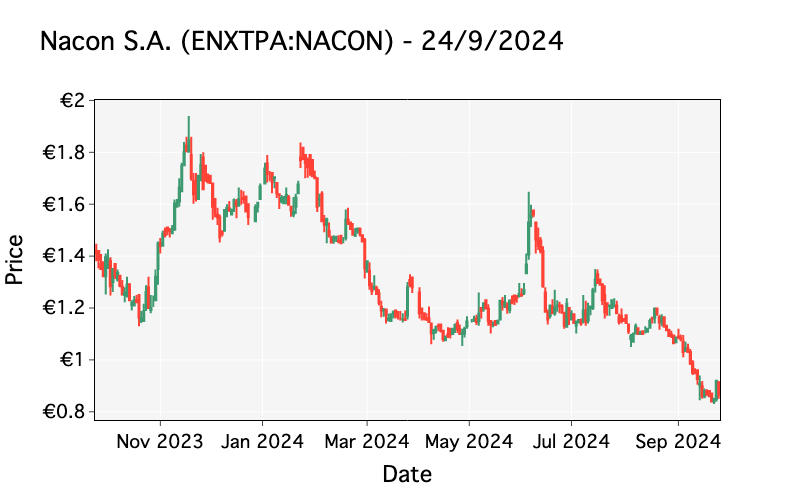
\includegraphics[width=\columnwidth]{France/images/Top_Returns/Top_1_candlestick.png}
    %\caption{Caption}
\end{figure}

\begin{figure}[H]
    \centering
    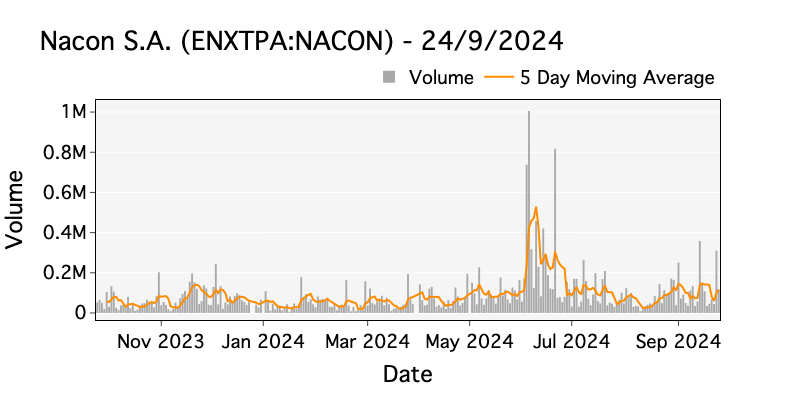
\includegraphics[width=\columnwidth]{France/images/Top_Returns/Top_1_volume.png}
    %\caption{Caption}
\end{figure}

\subsection*{Top 2}

\begin{figure}[H]
    \centering
    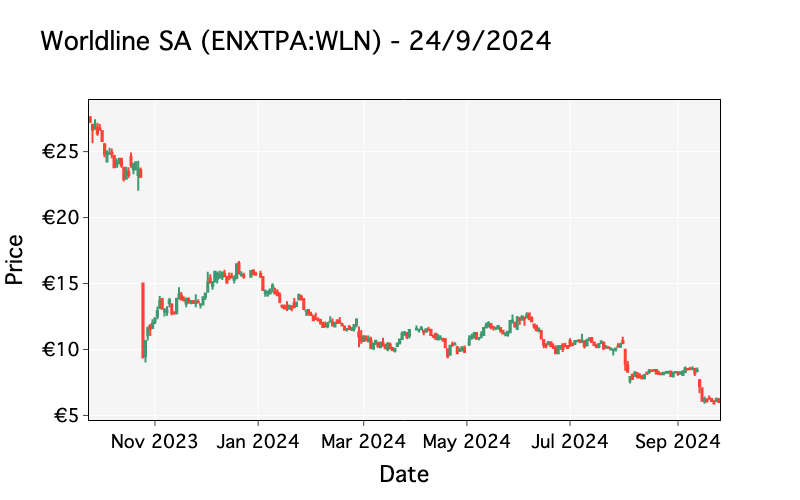
\includegraphics[width=\columnwidth]{France/images/Top_Returns/Top_2_candlestick.png}
    %\caption{Caption}
\end{figure}

\begin{figure}[H]
    \centering
    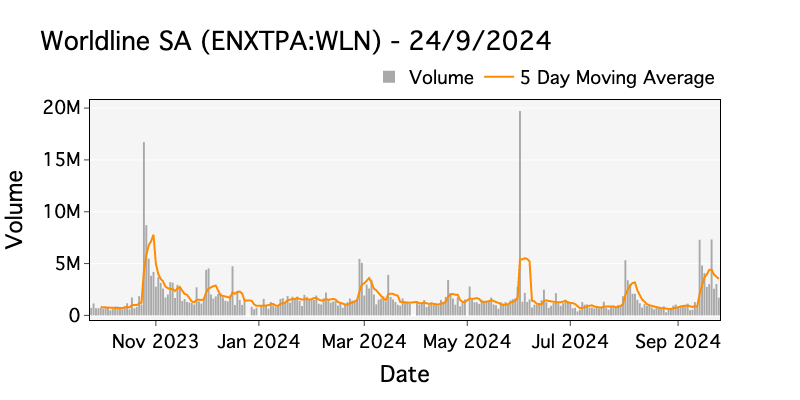
\includegraphics[width=\columnwidth]{France/images/Top_Returns/Top_2_volume.png}
    %\caption{Caption}
\end{figure}

\subsection*{Top 3}

\begin{figure}[H]
    \centering
    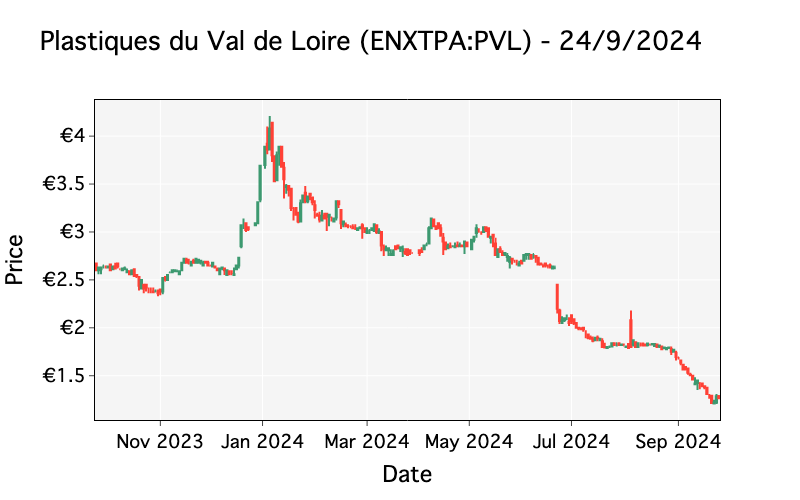
\includegraphics[width=\columnwidth]{France/images/Top_Returns/Top_3_candlestick.png}
    %\caption{Caption}
\end{figure}

\begin{figure}[H]
    \centering
    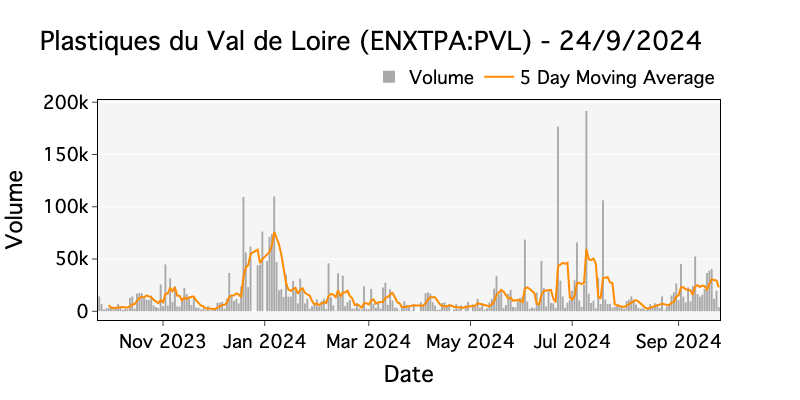
\includegraphics[width=\columnwidth]{France/images/Top_Returns/Top_3_volume.png}
    %\caption{Caption}
\end{figure}

\subsection*{Top 4}

\begin{figure}[H]
    \centering
    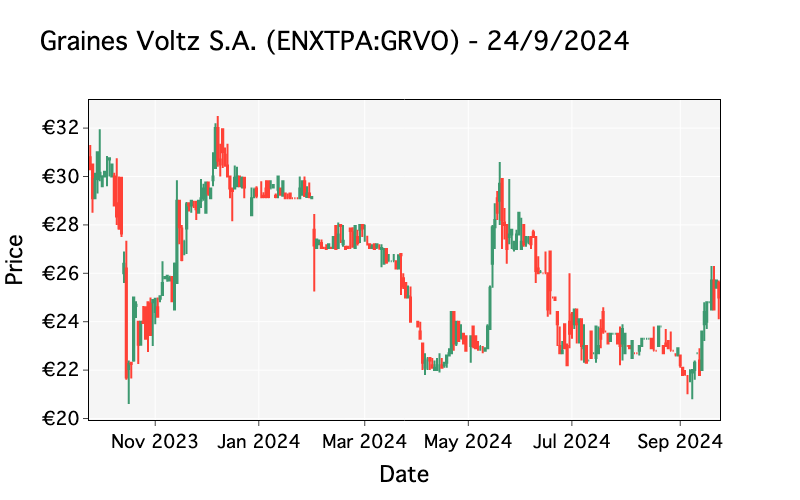
\includegraphics[width=\columnwidth]{France/images/Top_Returns/Top_4_candlestick.png}
    %\caption{Caption}
\end{figure}

\begin{figure}[H]
    \centering
    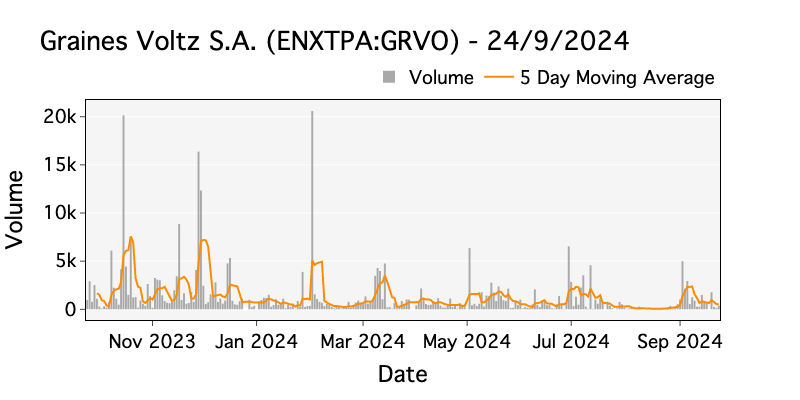
\includegraphics[width=\columnwidth]{France/images/Top_Returns/Top_4_volume.png}
    %\caption{Caption}
\end{figure}

\subsection*{Top 5}

\begin{figure}[H]
    \centering
    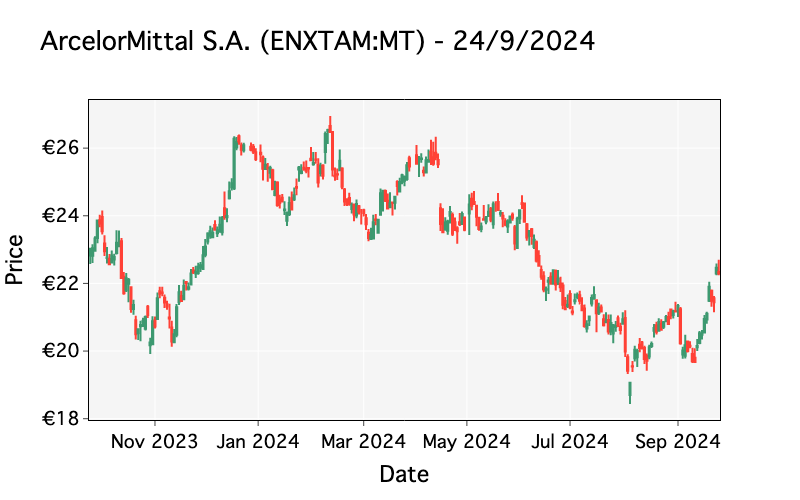
\includegraphics[width=\columnwidth]{France/images/Top_Returns/Top_5_candlestick.png}
    %\caption{Caption}
\end{figure}

\begin{figure}[H]
    \centering
    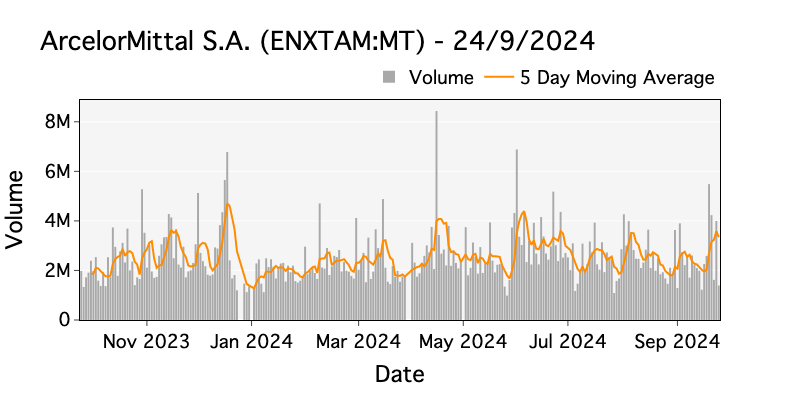
\includegraphics[width=\columnwidth]{France/images/Top_Returns/Top_5_volume.png}
    %\caption{Caption}
\end{figure}


\newpage
\section*{Worst performers}

\subsection*{Bottom 1}

\begin{figure}[H]
    \centering
    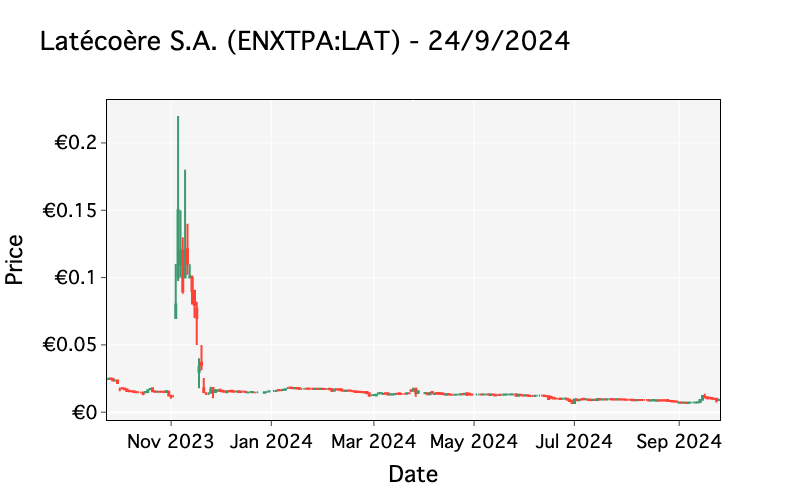
\includegraphics[width=\columnwidth]{France/images/Bottom_Returns/Bottom_1_candlestick.png}
    %\caption{Caption}
\end{figure}

\begin{figure}[H]
    \centering
    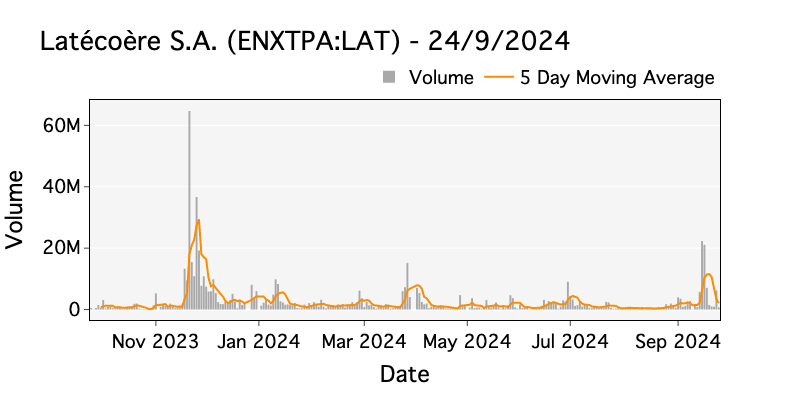
\includegraphics[width=\columnwidth]{France/images/Bottom_Returns/Bottom_1_volume.png}
    %\caption{Caption}
\end{figure}

\subsection*{Bottom 2}

\begin{figure}[H]
    \centering
    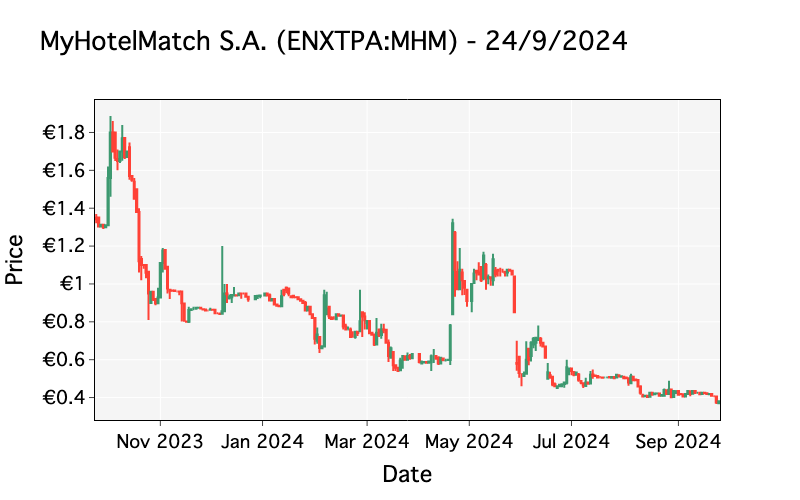
\includegraphics[width=\columnwidth]{France/images/Bottom_Returns/Bottom_2_candlestick.png}
    %\caption{Caption}
\end{figure}

\begin{figure}[H]
    \centering
    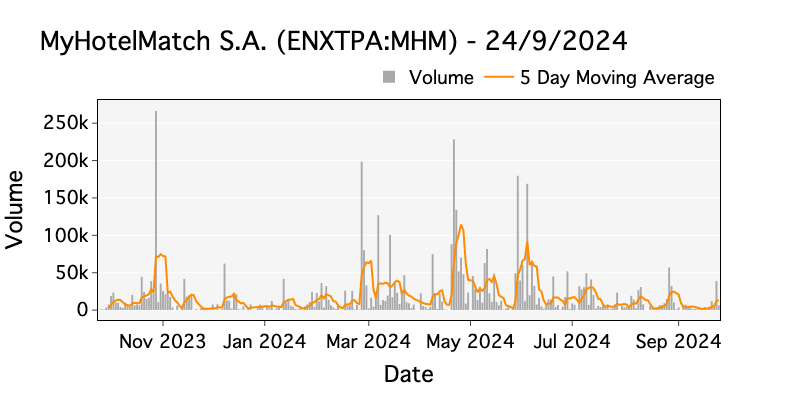
\includegraphics[width=\columnwidth]{France/images/Bottom_Returns/Bottom_2_volume.png}
    %\caption{Caption}
\end{figure}

\subsection*{Bottom 3}

\begin{figure}[H]
    \centering
    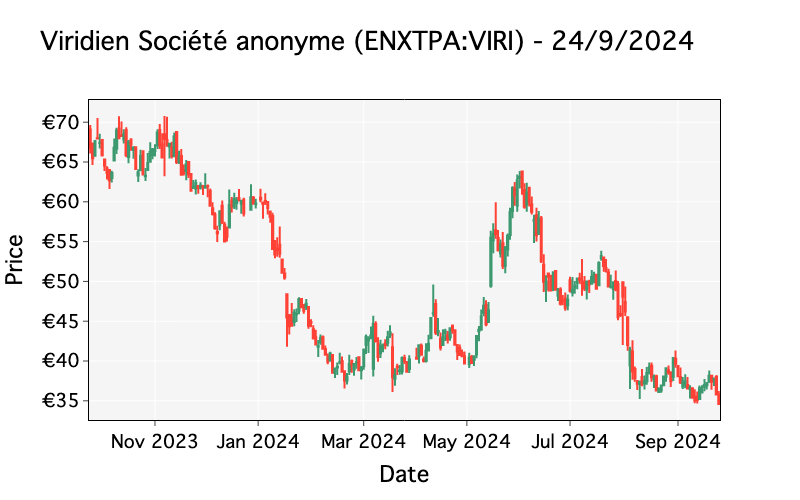
\includegraphics[width=\columnwidth]{France/images/Bottom_Returns/Bottom_3_candlestick.png}
    %\caption{Caption}
\end{figure}

\begin{figure}[H]
    \centering
    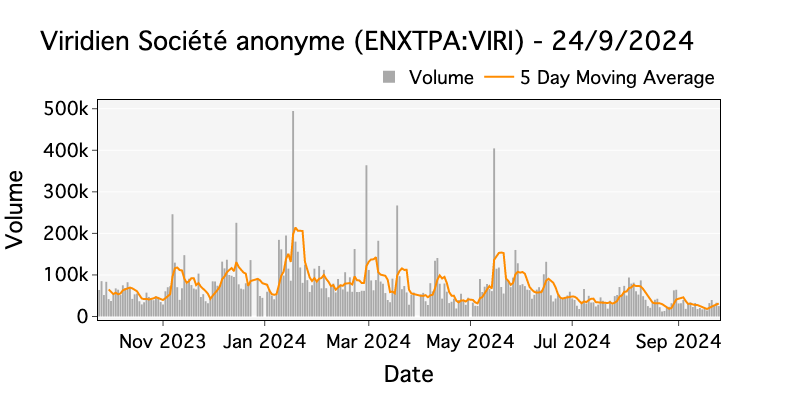
\includegraphics[width=\columnwidth]{France/images/Bottom_Returns/Bottom_3_volume.png}
    %\caption{Caption}
\end{figure}

\subsection*{Bottom 4}

\begin{figure}[H]
    \centering
    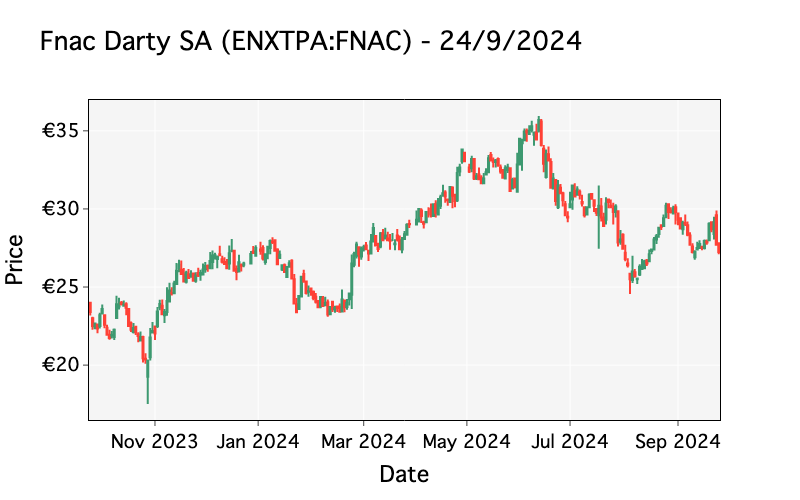
\includegraphics[width=\columnwidth]{France/images/Bottom_Returns/Bottom_4_candlestick.png}
    %\caption{Caption}
\end{figure}

\begin{figure}[H]
    \centering
    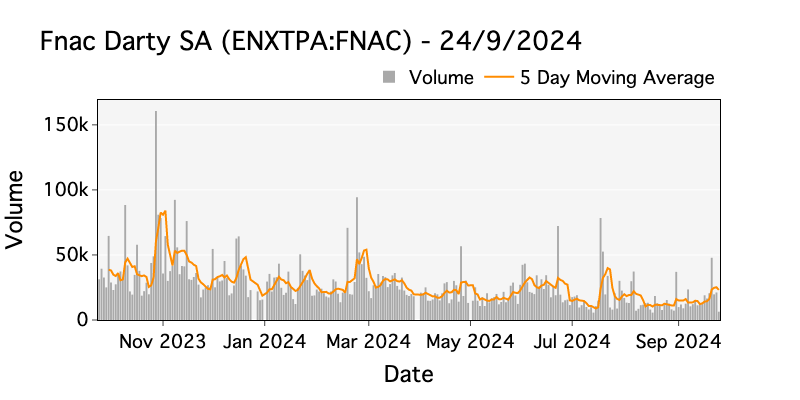
\includegraphics[width=\columnwidth]{France/images/Bottom_Returns/Bottom_4_volume.png}
    %\caption{Caption}
\end{figure}

\subsection*{Bottom 5}

\begin{figure}[H]
    \centering
    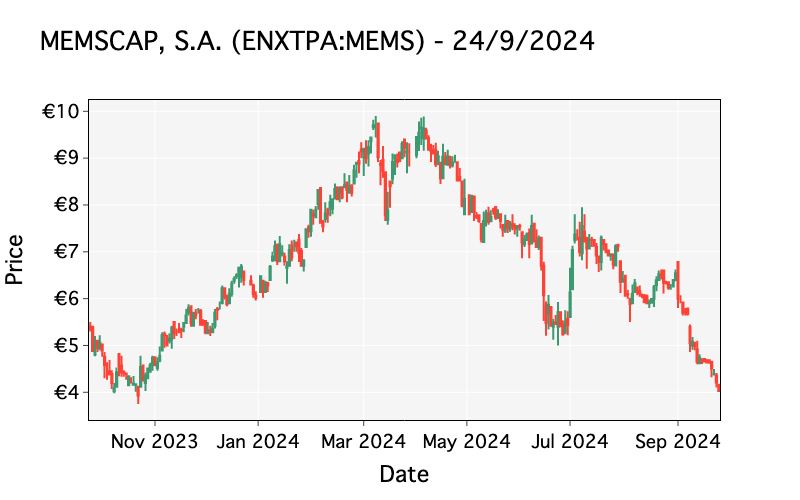
\includegraphics[width=\columnwidth]{France/images/Bottom_Returns/Bottom_5_candlestick.png}
    %\caption{Caption}
\end{figure}

\begin{figure}[H]
    \centering
    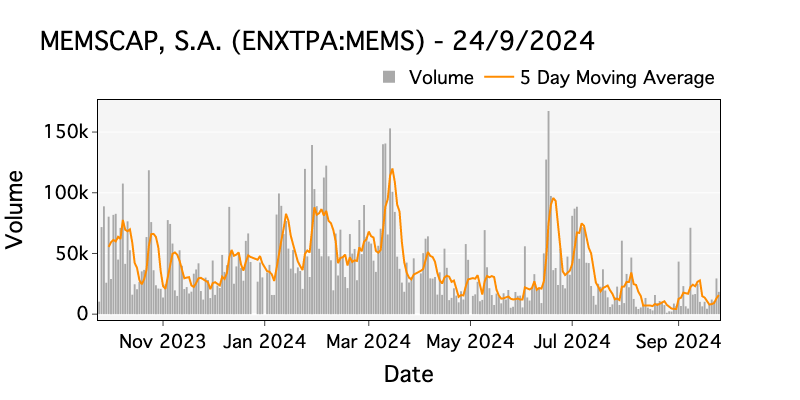
\includegraphics[width=\columnwidth]{France/images/Bottom_Returns/Bottom_5_volume.png}
    %\caption{Caption}
\end{figure}



\newpage
\section*{Largest relative volume}
\subsection*{Top 1}

\begin{figure}[H]
    \centering
    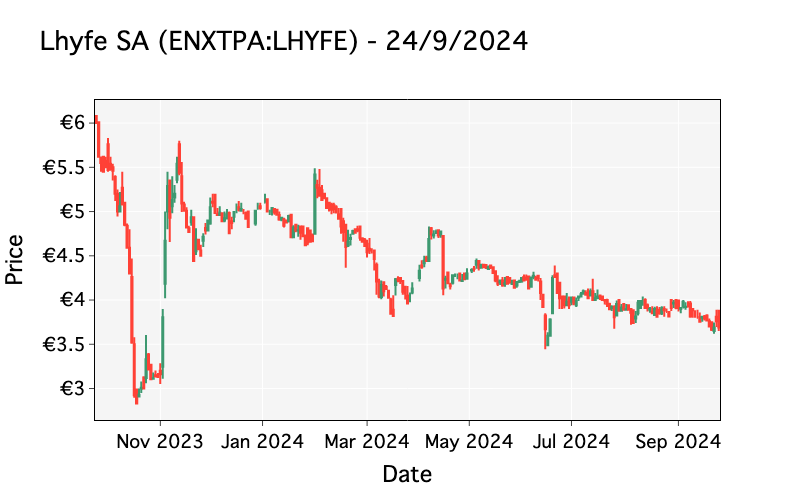
\includegraphics[width=\columnwidth]{France/images/Top_Volume/Top_1_candlestick.png}
    %\caption{Caption}
\end{figure}

\begin{figure}[H]
    \centering
    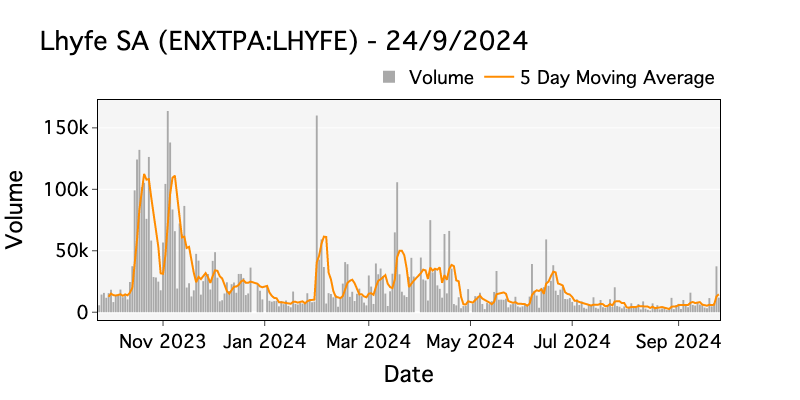
\includegraphics[width=\columnwidth]{France/images/Top_Volume/Top_1_volume.png}
    %\caption{Caption}
\end{figure}

\subsection*{Top 2}

\begin{figure}[H]
    \centering
    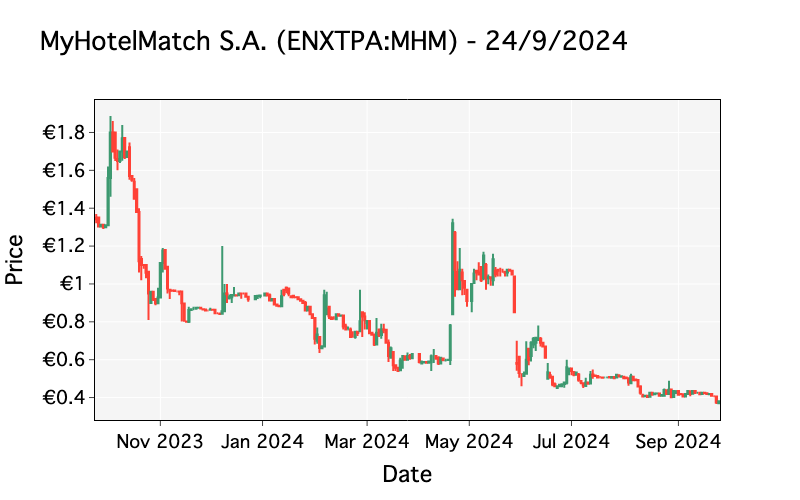
\includegraphics[width=\columnwidth]{France/images/Top_Volume/Top_2_candlestick.png}
    %\caption{Caption}
\end{figure}

\begin{figure}[H]
    \centering
    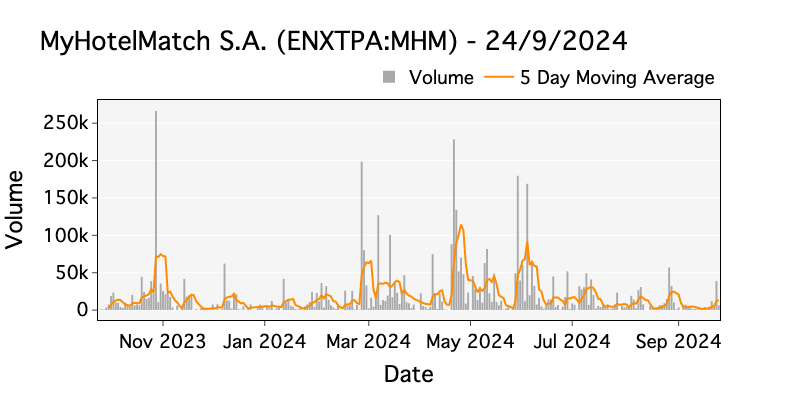
\includegraphics[width=\columnwidth]{France/images/Top_Volume/Top_2_volume.png}
    %\caption{Caption}
\end{figure}

\subsection*{Top 3}

\begin{figure}[H]
    \centering
    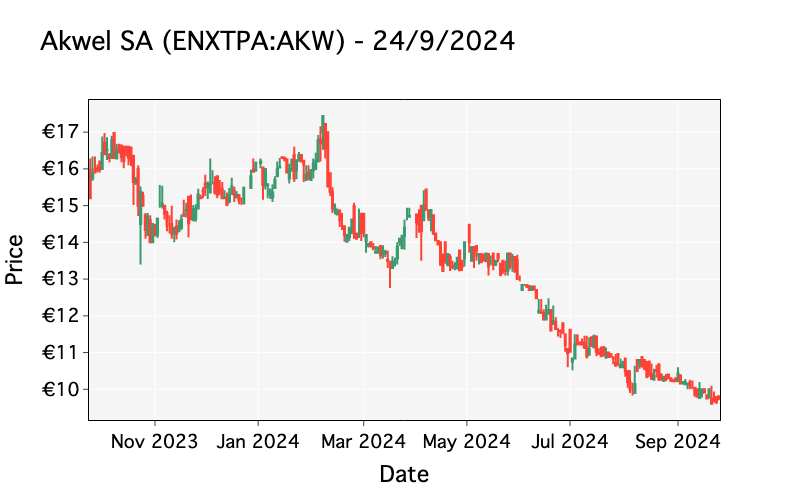
\includegraphics[width=\columnwidth]{France/images/Top_Volume/Top_3_candlestick.png}
    %\caption{Caption}
\end{figure}

\begin{figure}[H]
    \centering
    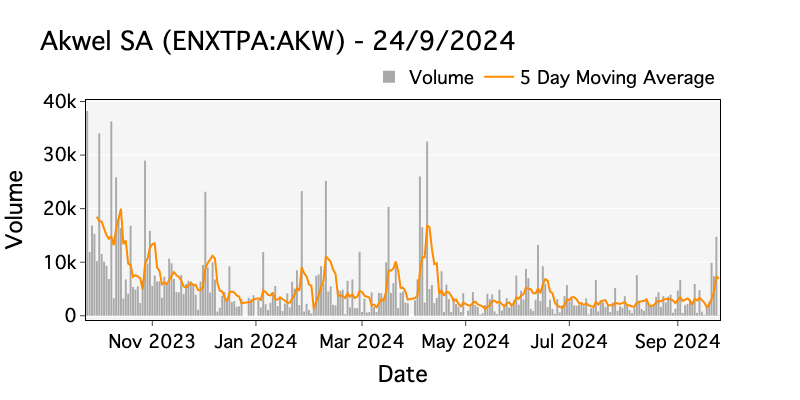
\includegraphics[width=\columnwidth]{France/images/Top_Volume/Top_3_volume.png}
    %\caption{Caption}
\end{figure}

\subsection*{Top 4}

\begin{figure}[H]
    \centering
    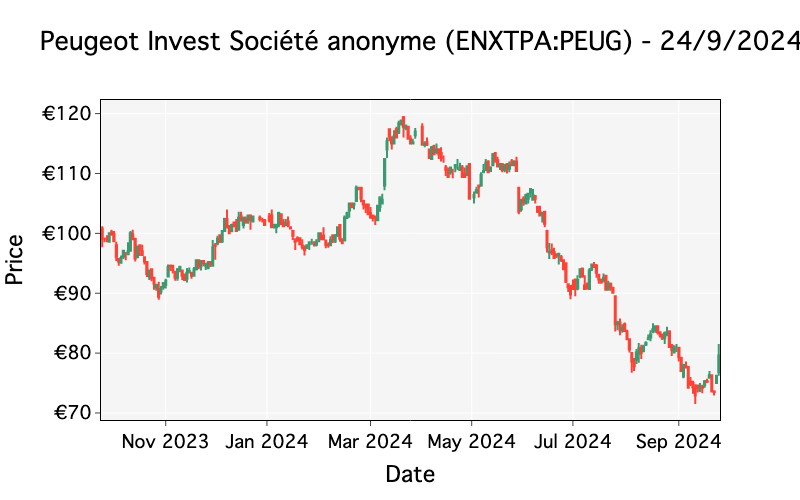
\includegraphics[width=\columnwidth]{France/images/Top_Volume/Top_4_candlestick.png}
    %\caption{Caption}
\end{figure}

\begin{figure}[H]
    \centering
    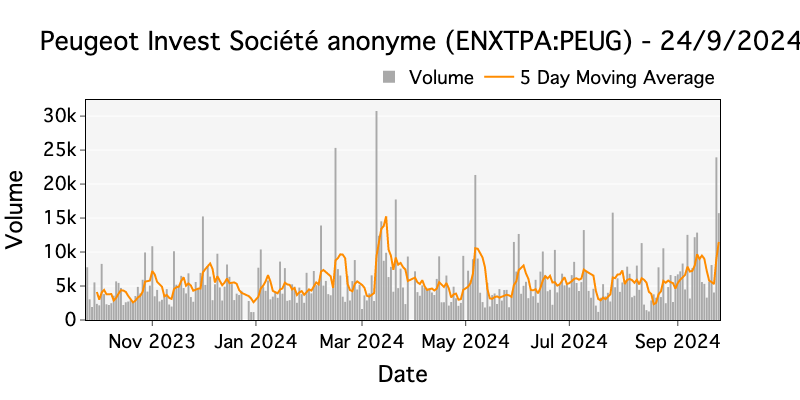
\includegraphics[width=\columnwidth]{France/images/Top_Volume/Top_4_volume.png}
    %\caption{Caption}
\end{figure}

\subsection*{Top 5}

\begin{figure}[H]
    \centering
    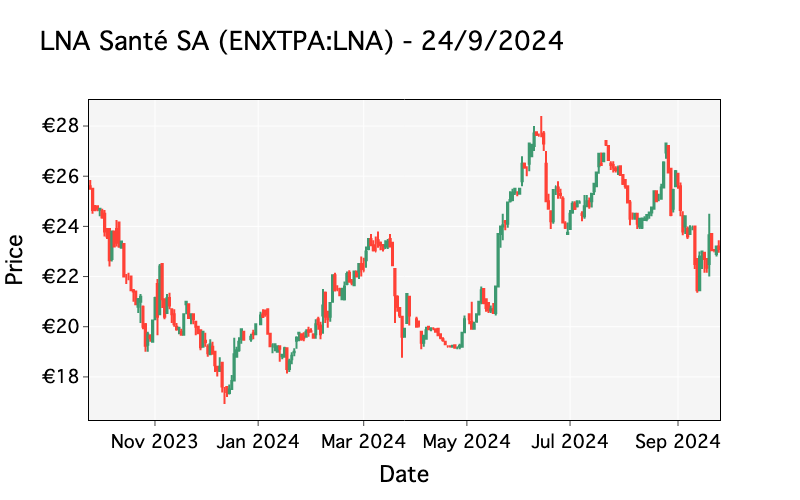
\includegraphics[width=\columnwidth]{France/images/Top_Volume/Top_5_candlestick.png}
    %\caption{Caption}
\end{figure}

\begin{figure}[H]
    \centering
    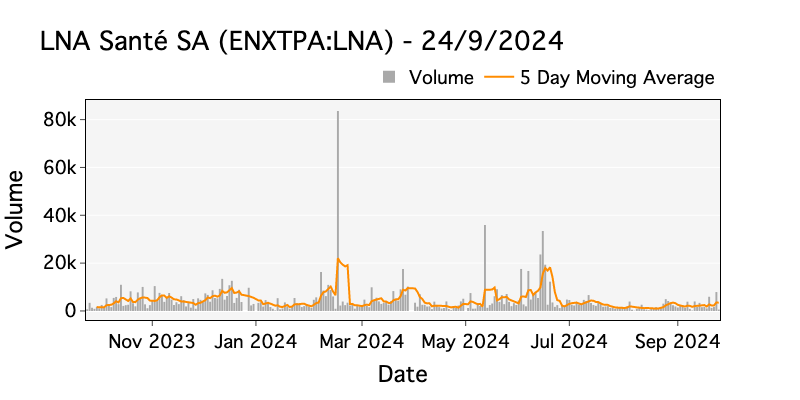
\includegraphics[width=\columnwidth]{France/images/Top_Volume/Top_5_volume.png}
    %\caption{Caption}
\end{figure}

\end{document}